%!TEX root = ../main.tex
% file: assignment2.tex

\graphicspath{{C:/Local_Files/GitHub/MCS507_Final_Project/tex/include/}}
%\graphicspath{{C:/Documents and Settings/amcelhinney/My Documents/GitHub/MCS507_Final_Project/tex/include}}
%\graphicspath{{C:/Documents and Settings/amcelhinney/My Documents/GitHub/MCS507--Project-3/tex/include/}}

\section{Assignment Three: A More Substantial Example} % (fold)
\subsection{Overview of Example} % (fold)
\begin{flushleft}We know consider the application of Bayesian Classifiers to a simple problem; determining whether an object is likely to be blue, green, or yellow based upon its position (Note that the shapes of the objects were added to provide additional visual distinction and do not represent another dimension of the data). The dots were created manually using the $Orange$ module's data painting feature. The groups were specifically chose such that they have unequal size and that there exists substantial overlap between the groups. 
\end{flushleft}

\begin{table}[H]
\caption{Overview of the Data Set}
\centering
\begin{tabular}{c c}
\hline\hline
Category & Count \\
\hline
Blue & 900 \\
Green & 630 \\
Yellow & 760 \\
\hline
\end{tabular}
\label{table:nonlin} 
\end{table}


\begin{flushleft}We begin our implementation by writing functions to split the data into separate lists for each class. This will be used later for graphing and scoring purposes. 
\end{flushleft}
\begin{lstlisting}[caption={Partition the Data},label=2nd,firstnumber=16]
########################
# Functions to split the data
########################


def unique(data, class_col):
    """
    Creates a list of unique observations from data
    class_col=the column number containing the group
    """
    groups=[]
    for i in range(len(data)):
        # Check to see if this group has been added to groups
        if data[i][class_col] not in groups:
            groups.append(data[i][class_col])
    return groups


# Split the data into unique groups
def unique_split(data,class_col):
    # Get the list of unique groups
    r=unique(data,class_col)
    p=[]
    for q in range(len(r)):
        p.append([])
    for i in range(len(data)):
        #print i
        for j in range(len(r)):
            #print j
            if data[i][class_col]==r[j]:
                p[j].append(data[i])

    return p
\end{lstlisting}

\begin{flushleft}Next, we import the data using the $C4.5$ data format. This format is common in machine learning as it provides definitions of the variables, as well as explicit type declarations that are understood by the majority of machine learning software tools.  We then split the data into the respective groups.
\end{flushleft}

\begin{lstlisting}[caption={Import the Data and Split},label=2nd,firstnumber=51]
data = orange.ExampleTable("3_groups")
print data.domain.attributes
print data[:4]

# Get a small amount of data
index=Orange.data.sample.SubsetIndices2(p0=0.10)
ind=index(data)
#data_test=data.select(ind,0)
data_test=data


########################
# Split the data
########################

X, Y = data_test.to_numpy("A/C")
data_2=[]
for i in range(len(Y)):
    data_2.append([X[i][0],X[i][1],Y[i]])
p=unique_split(data_2,2)

# Group 1
X11=[p[0][i][0] for i in range(len(p[0]))]
X12=[p[0][i][1] for i in range(len(p[0]))]

# Group 2
X21=[p[1][i][0] for i in range(len(p[1]))]
X22=[p[1][i][1] for i in range(len(p[1]))]

# Group 3
X31=[p[2][i][0] for i in range(len(p[2]))]
X32=[p[2][i][1] for i in range(len(p[2]))]

# Obtain the counts
len(X11);len(X21);len(X31)

\end{lstlisting}

\begin{flushleft}Next, we prepare the data into the form required by $Matplotlib$ and plot the data.
\end{flushleft}

\begin{lstlisting}[caption={Prepare the Data for Plotting; Plot the Data},label=2nd,firstnumber=87]
########################
# Plot the data
########################


import matplotlib.pyplot as plt
import matplotlib
fig = plt.figure()
ax1 = fig.add_subplot(111)

ax1.scatter(X11, X12, s=10, c='b', marker="+")
ax1.scatter(X21, X22, s=10, c='c', marker="o")
ax1.scatter(X31, X32, s=10, c='y', marker="x")
plt.title('Plot of Three Classes of Data')
plt.show()

\end{lstlisting}

\begin{figure}[H]
    \centering
       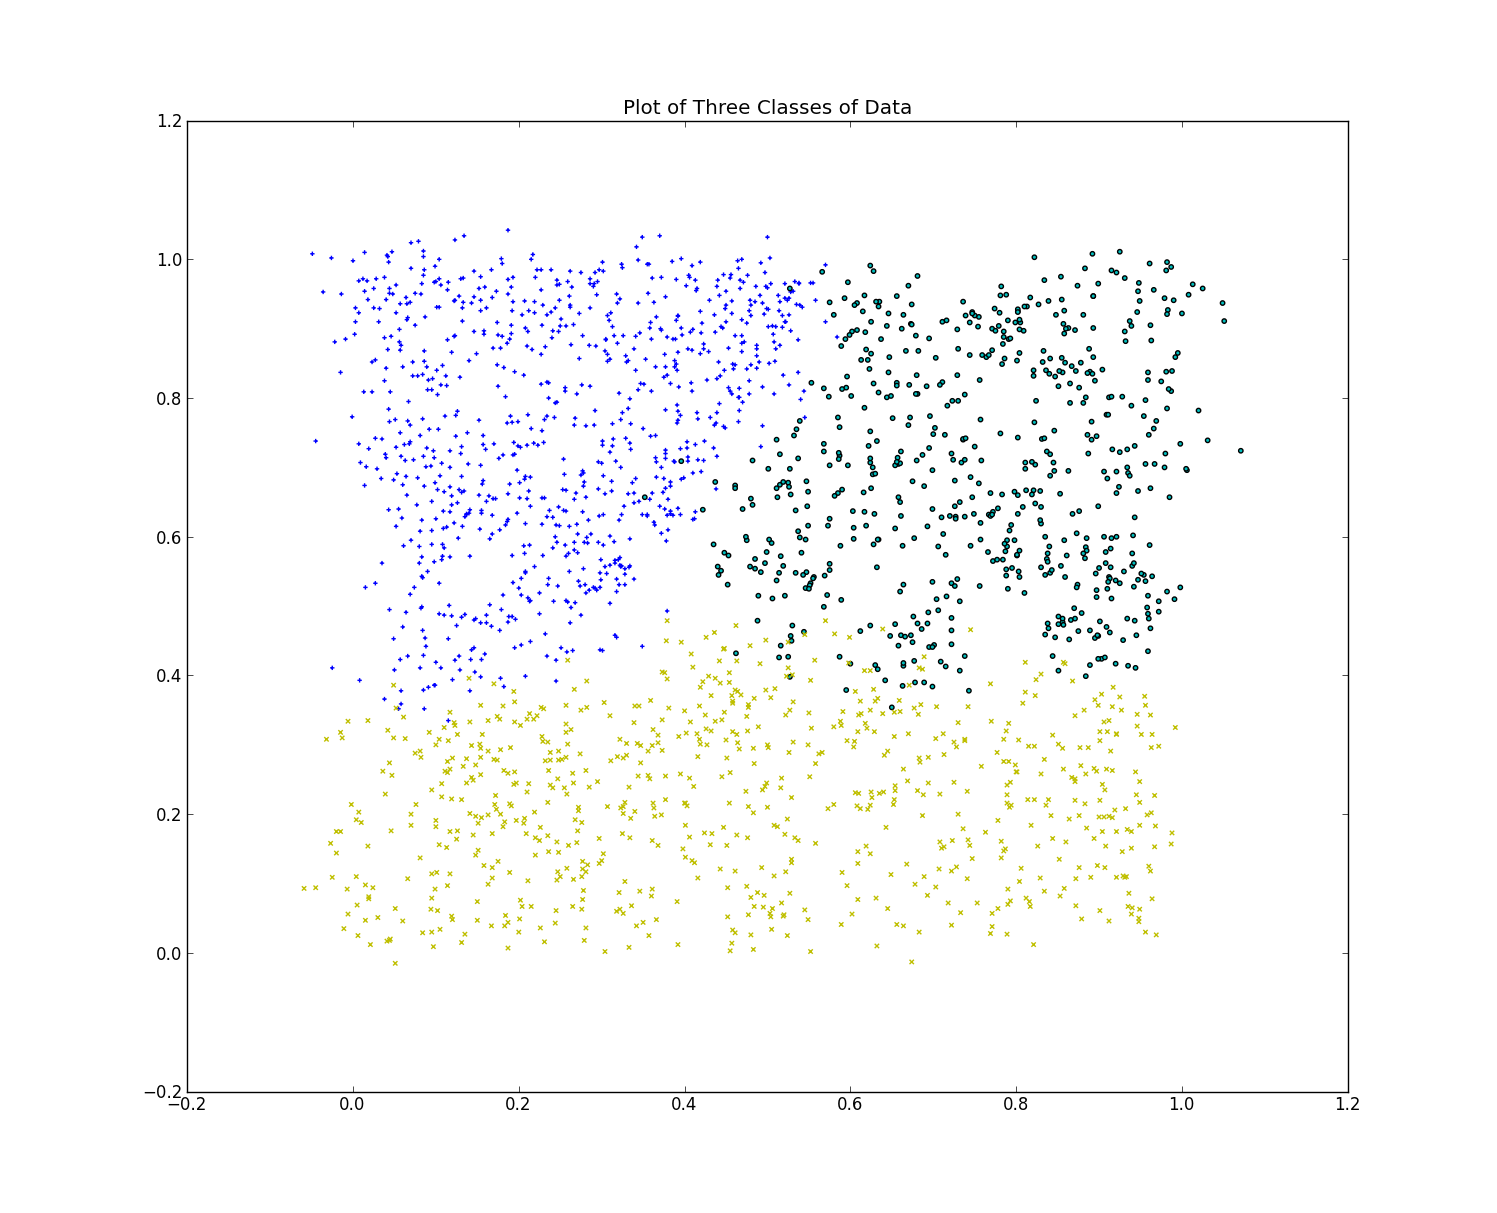
\includegraphics[width=6.5 in]{3_groups.png}
    \caption{Classification of 3 colors in 2-dimensional space}
    \label{Example Data}
\end{figure}


\begin{flushleft}Using the Bayesian methods outlined in the first section, a Naive Bayes Classifier was trained and validated using k-fold cross validation.
\end{flushleft}

\begin{lstlisting}[caption={Construct the Classifier},label=2nd,firstnumber=103]
########################
# Build Classifier
########################

import orange, orngTest, orngStat, orngTree   
classifier = orange.BayesLearner(data)
bayes = orange.BayesLearner()
bayes.name = "bayes"
learners = [bayes]

results = orngTest.crossValidation(learners, data_test, folds=10)
\end{lstlisting}

\begin{flushleft}Once the classifier is constructed, we wish to compute the misclassified operations. The package $Orange$ provides a convenient way of doing this, however it cannot interface directly with $Matplotlib$. Thus, the data was converted to $NumPy$ arrays.
\end{flushleft}

\begin{lstlisting}[caption={Compute the Misclassified Observations},label=2nd,firstnumber=115]
########################
# Compute the misclassified observations
########################

X, Y = data_test.to_numpy("A/C")
data_scored=[]
for i in range(len(results.results)):
    if results.results[i].classes[0]==results.results[i].actual_class:
        data_scored.append(1)
    else:
        data_scored.append(0)

import matplotlib.pyplot as plt
import matplotlib

X1w=[];X2w=[]
for i in range(len(X)):
    if data_scored[i]==0:
        X1w.append(X[i][0])
        X2w.append(X[i][1])
\end{lstlisting}

\begin{flushleft}We now overlay the misclassified observations onto plots of the data points to give a visual approximation of how successful is our classifier.
\end{flushleft}

\begin{lstlisting}[caption={Compute the Misclassified Observations},label=2nd,firstnumber=123]
########################
# Plot the misclassified data
########################
fig = plt.figure()
ax1 = fig.add_subplot(111)

ax1.scatter(X11, X12, s=10, c='b', marker="+")
ax1.scatter(X21, X22, s=10, c='c', marker="o")
ax1.scatter(X31, X32, s=10, c='y', marker="x")
ax1.scatter(X1w, X2w, s=10, c='m', marker="^")
plt.title('Plot of Three Classes of Data, Showing the Misclassified Elements')
plt.show()
\end{lstlisting}

\begin{figure}[H]
    \centering
       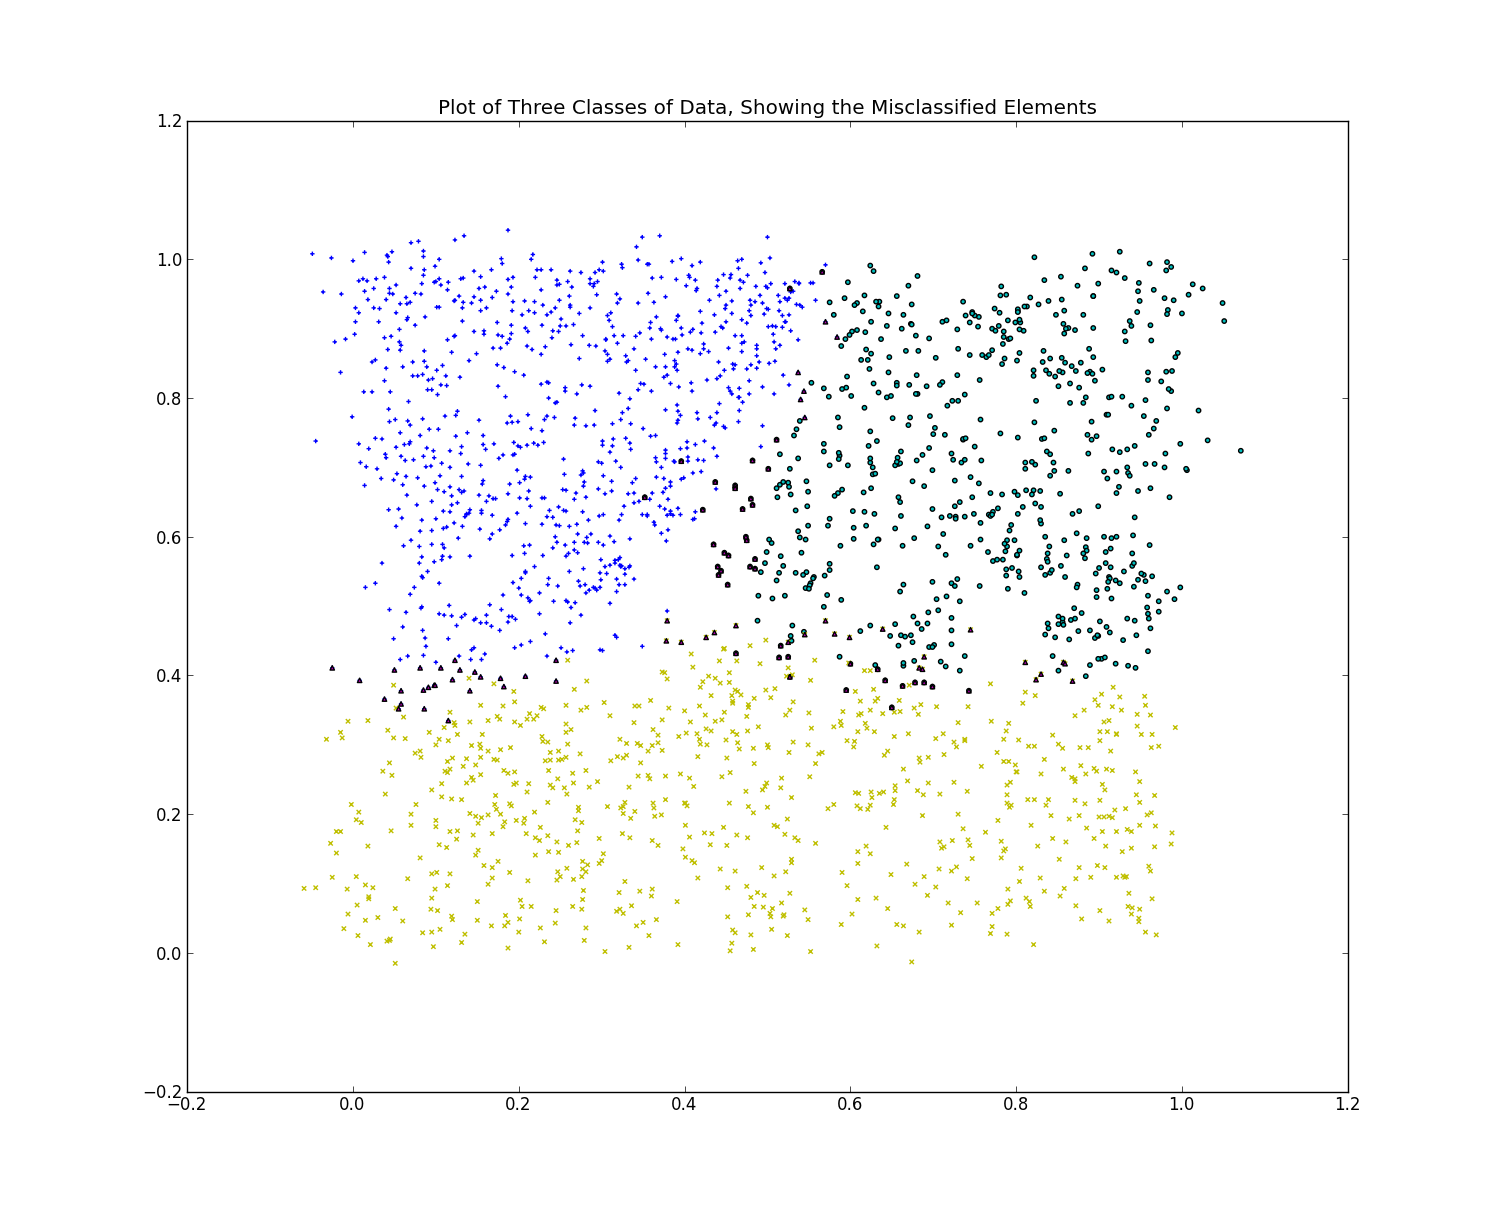
\includegraphics[width=6.5 in]{3_groups_mis.png}
    \caption{Classification of 3 colors in 2-dimensional space; Misclassifications displayed}
    \label{Example Data}
\end{figure}

\begin{flushleft}As the above figure shows, our classifier is quite successful. We see a small number of misclassified observations (represented as dark triangles) that predictably lie in the boundaries between the three groups. However, in addition to a visual representation of the accuracy of the classifier, the $Orange$ package provides us with a full range of summary statistics to assess the model performance. 
\end{flushleft}
\begin{lstlisting}[caption={Compute the Misclassified Observations},label=2nd,firstnumber=151]
# output the results
print "Learner CA IS Brier AUC"
for i in range(len(learners)):
    print "%-8s %5.3f %5.3f %5.3f %5.3f" % (learners[i].name, \
    orngStat.CA(results)[i], orngStat.IS(results)[i], orngStat.BrierScore(results)[i], orngStat.AUC(results)[i])
\end{lstlisting}

\begin{table}[H]
\caption{Model Performance Statistics}
\centering
\begin{tabular}{c c}
\hline\hline
Statistics & Value\\
\hline
Classification Accuracy & 96\% \\
Information Score & 1.301\\
Brier Score & .093\\
Area Under ROC &.998\\
\hline
\end{tabular}
\label{table:nonlin} 
\end{table}

\begin{flushleft}The exact definitions of all of these metrics is beyond the scope of this paper. However, one metric to call out is the Classification Accuracy. This is simply the percentage of observations that are classified correctly. The value of 96\% represents an excellent classifier. This intuitively matches our observations based on the graph of misclassifications.
\end{flushleft}

% subsection Overview of Example (end)




% section Assignment One: Overview and Illustrative Example (end)
